\chapter{Entwicklung}
In diesem Kapitel werden die einzelnen Komponenten, die für eine komplette Ingestion notwendig sind entwickelt.
Nach \citeauthor{DL-Ing-Mgmt} ist der Ingestion-Prozess eines Data-Lake-Systems, als erster Schritt im Lebenszyklus der Daten, maßgebend dafür, wie gut die Daten später verwendet und verarbeitet werden können.
Dafür sollte das System einige Herausforderungen erfüllen.
Diese sind die Unterstützung für strukturiert, teil-strukturiert und unstrukturierte Datenquellen und die Möglichkeit für einmalige oder kontinuierliche Ingestion.
Zu dem zweiten Punkt gehört außerdem, dass geänderte Daten mit einer Datenversionierung im Data Lake gespeichert werden können.
Zur Erfüllung dieser Herausforderungen und um allgemein gut mit den Daten interagieren zu können, sollte sich die Ingestion zusätzlich um die Erstellung von Metadaten kümmern.

Das zu entwickelnde System lässt sich in die drei Teile Ingestion, Delta-Erkennung und Datenversionierung unterteilen.
Bei der Ingestion soll der Teil entwickelt werden, der dafür verantwortlich ist, Daten aus verschiedensten Quellen in das Data-Lake-System zu laden und zu speichern.
Die Delta-Erkennung ist ein Mechanismus, der dafür sorgen soll, dass bei einer kontinuierlichen Ingestion nur geänderte Daten neu in das System integriert werden.
Zum Schluss hat die Datenversionierung das Ziel, geänderte Daten im Data Lake so zu verwalten, dass Analysen über den Verlauf der Daten und Abfragen älterer Version möglich werden.

\section{Vorüberlegungen}

\subsection{Datenquellen}
Ein Kernpunkt für die Entwicklung der Ingestion-Schnittstelle ist die Analyse der möglichen Datenquellen.
Da das System alle möglichen Datenquellen unterstützen soll, werden hier mögliche Typen dargestellt, mit denen sich alle Datenquellen abdecken lassen.
Dazu werden Merkmale betrachtet die Art und der Typ Ingestion bestimmen.
Mit der Art wird hier bezeichnet, ob die verwendeten Daten strukturiert, semi- oder unstrukturiert sind.
Da in der Vorarbeit, dem Masterprojekt, \textit{Apache Spark} verwendet wurde, ist dieser Punkt bereits abgedeckt und fällt bei der Entwicklung nicht weiter ins Gewicht.

Als zweites gibt es die Typen, die hier beschreiben, wie Daten in das System gelangen.
Dazu gibt es zwei Merkmale, in denen sich die Ingestions unterscheiden können.
Das erste ist, ob die Unterscheidung zwischen Push- und Pull-Prinzip.
Bei dem Push-Prinzip werden die zu speichernden Daten mit der Anfrage an das System gesendet und bei dem Pull-Prinzip muss dass System die Daten aus einer Quelle laden.
Die zweite Unterscheidung findet statt in einmalige in kontinuierliche Ingestion.
Diese Unterscheidungen können, müssen aber nicht, von der Datenquelle abhängig sein.
Als Beispiel gibt es Datenströme, die laufend Daten senden und somit eine Ingestion benötigen, die auch laufend Daten annimmt.
Im Gegensatz dazu gibt es Datenbanken, bei denen das System die Daten aus der Quelle laden muss und somit die Ingestion sowohl einmalig als auch kontinuierlich sein kann.

Aus diesen Unterscheidungen ergeben sich die vier mögliche Verarbeitungswege, die in \ref{fig:ingestion_types} zu sehen sind.
Sowohl für Push- und Pull-Prinzip kann eine einfache Ingestion ausgeführt werden, die sich für kontinuierliche Pull-Ingestions wiederholt.
Bei einer kontinuierlichen Ingestion, bei der Daten an das System gesendet werden, handelt es sich um Datenströme, die eine extra Verarbeitung erfordern.

\begin{figure}
    \centering
    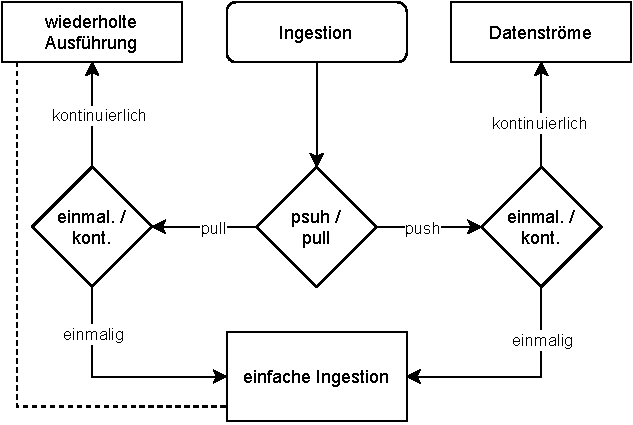
\includegraphics{Grafiken/ingestion-types.pdf}
    \caption{Ingestion-Typen}
    \label{fig:ingestion_types}
\end{figure}

\subsection{Architektur Ansatz}
Die Anwendung, die im Masterprojekt entwickelt wurde ist eine monolithische Anwendung.
Das bedeutet, dass die gesamte Software als ein großes Programm entwickelt und bereitgestellt wird.
Solche Anwendungen sind zwar in der Entwicklung und Bereitstellung leicht umzusetzen, haben aber größere Nachteile in Bereichen wie Fehlertoleranz und Wartung.
Im Vergleich dazu gibt es die Microservice-Architektur, bei der mehrere kleine Anwendungen entwickelt werden, die bestimmte aufgaben übernehmen und am gesamt Problem gemeinsam beteiligt sind.
Diese haben im, wie von \textcite{microservices} dargestellt, mehrere Vorteile gegenüber monolithischen Anwendungen.
Die Wartung fällt bei vielen kleinen Programmen leichter, da sie übersichtlicher und verständlicher sind als ein großes und Fehler betreffen jeweils nur den Microservice selbst.
Außerdem ist es einfacher bestimmte Aspekte der Software zu skalieren und bei Updates bleibt eine höhere Verfügbarkeit, da nur ein kleiner Teil des Systems neu gestartet werden muss.

Als Nachteil wird aber auch erwähnt, dass die Bereitstellung einer Mircoservice-Architektur komplexer ist als die einer monolithischen.
Diese Problem kann aber mit Container-Lösung wie \textit{Docker}\footnote{https://www.docker.com/} vereinfacht werden.
Dabei werden sogenannte Contianer aus den Mircoservices gebaut, die ähnlich zu einer virtuellen Maschine sind und einen bestimmten Zustand speichern.
Beim Starten eines Containers wird genau in diesem Zustand eingestiegen, so dass man ohne großen Aufwand zum Beispiel einen Webserver mit einer bestimmt Anwendung auf verschiedenen System starten kann, ohne sich um deren Installationen kümmern zu müssen.

Auf Grund der genannten Vorteile soll das Data Lake System und damit die Ingestion als Microservice-Architektur entwickelt werden.
Das bedeutet, dass Punkte gefunden werden müssen, an denen sich das System gut in einzelene Anwendungen trennen lässt.

\section{Ingestion}
Bei der Entwicklung der Ingestion wird das Laden der Daten und die Architektur der Anwendung betrachtet.
Es wird eine Datenmodell, in dem die Informationen zu den Datenquellen gespeichert werden, der Ablauf der verschiedenen Ingestion-Prozesse und die Kommunikation zwischen den einzelnen Mircoservices entwickelt.

\subsection{Server Architektur}
\label{sec:arch}

\begin{figure}
    \centering
    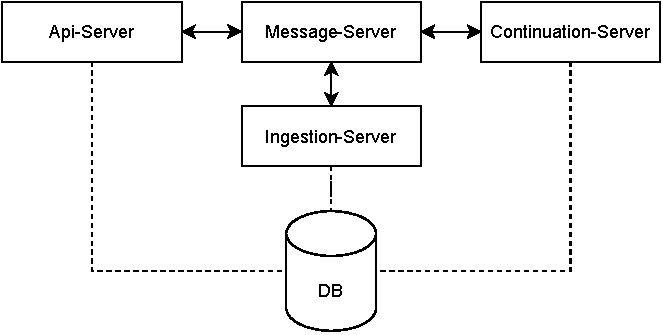
\includegraphics{Grafiken/ingestion-arch.pdf}
    \caption{Architektur der Ingestion Komponenten}
    \label{fig:ingestion_arch}
\end{figure}

Für die Umsetzung der Mircoservice-Architektur wird die Ingestion in Komponenten aufgeteilt, die \fref{fig:ingestion_arch} zu sehen sind.
Es gibt drei Services, die für die Ingestion spezifischen Aufgaben zuständig sind, eine Datenbank, in der die Informationen über Datenquellen gespeichert werden und einen Service, der für die Kommunikation verantwortlich ist.
Der \textbf{Api-Server} bietet einen REST-Schnittstelle, über die man mit der Ingestion interagieren kann.
Hier werden die Endpunkte aus \fref{tab:enpoints} benötigt, die die Schnittstellen zur Verwaltung von Datenquellen und das Ausführen von Ingestions bereitstellen.
Außerdem ist er dafür zuständig, die empfangenen Informationen über Datenquellen in der Datenbank zu verwalten.
der \textbf{Continuation-Server} überprüft regelmäßig alle kontinuierlichen Datenquellen, ob diese eine Zeitsteuerung haben und aktuell ausgeführt werden sollten.
Der \textbf{Ingestion-Server} ist die Anwendung, die die eigentliche Ingestion ausführt.
Dafür wartet dieser auf eine Aufforderung durch entweder den Api- oder den Continuation-Server.

\begin{table}[!ht]
    \centering
    \begin{tabular}{| l | l | p{3in} |}
        \hline
        Pfad                                        & HTTP-Methode  & Beschreibung \\
        \hline \hline
        /datasources                                & GET           & Liefert alle im System gespeicherten Datenquellen \\
        \hline
        /datasources/\textless id\textgreater       & GET           & Liefert die Datenquelle mit der im Pfad übergebenen Id \\
        \hline
        /datasources                                & POST          & Erstellt eine neue Datenquelle \\
        \hline
        /datasources/\textless id\textgreater       & PUT           & Bearbeitet die Daten Datenquelle mit der im Pfad übergebenen Id \\
        \hline
        /datasources/\textless id\textgreater/run   & GET           & Startet eine Ingestion der Datenquelle mit der im Pfad übergebenen Id \\
        \hline
    \end{tabular}
    \caption{Endpunkte des Api-Servers}
    \label{tab:enpoints}
\end{table}

\subsection{Plugins}
Da bei manchen Ingestions nicht immer ein festgelegtes Vorgehen ausreicht, um die Daten aus bestimmten Datenqellen zu laden, muss ein System entwickelt werden, wie möglichst ohne großen Aufwand die Inegstion erweitert werden kann.
Beispiele für solche Fälle sind die Verarbeitung von Datenströmen oder die Ingestion von Daten aus APIs, die nicht generallisiert werden können.
Als Lösung für das Problem, können Plugins der Datenquelle hinzugefügt werden. 
Diese Plugins sollen Logik enthalten, die an verschiedenen Stellen der Ingestion ausgeführt werden sollen.
Aktuell sind diese Stellen das Laden der Daten, nach dem Laden der Daten und die Stream-Verarbeitung.
Dabei ist zu beachten, dass Plugins, die das Laden der Daten abhandeln, das Standardverhalten des Ingestion-Servers überschreiben und das Stream-Verarbeitung nur mit Plugins möglich ist.
Damit es nicht zu Konflikten bei Abhängigkeiten der Plugins gibt, muss der Ingestion-Server eine Mechanik implementieren, bei der die Abhängigkeiten der Plugins für jede Datenquelle dynamisch gealden werden.

\subsection{Datenquellen}
Eine letzte Vorüberlegung für die Ingestion ist, welche Informationen erfasst werden müssen, um eine generische Ingestion zu ermöglichen.
Da es keine klaren Parameter wie zum Beispiel Datenbanknamen oder IP-Adressen gibt, die bei allen Quellen gleich sind, orientiert sich die Eingabe an der Funktionsweise von \textit{Pyspark / Apache Spark}.
Um festzulegen, woher Daten gelesen werden sollen, kann man beim erstellen einer \verb|SparkSession| einmal das Format der zu lesenden Daten angeben.
Außerdem bietet die \verb|SparkSession| die Funktion Maven-Abhängigkeiten hinzuzufügen, die Unterstützung für verschiedene Formate bringen.
Bei den meisten Formaten müssen zusätzlich noch Optionen gesetzt werden, die zum Beispiel Verbindungsparameter oder Lesemodus enthalten.
Diese Optionen sind eine Sammlung von Schlüssel-Wert-Paaren.
Eine Ausnahme besteht hierbei bei der Optionen, für die Quelledateien bei Datei-Ingestions, da diese automatisch durch die Anwendung gesetzt wird.
Daraus lassen sich bereits drei Felder ableiten, die in einem Datenmodell für die Datenquellen enthalten sein müssen: Format, Pakete und Optionen.

Neben den \textit{Spark}-spezifischen Feldern soll die Datenquelle auch die anwendungsspezifischen Informationen enhalten.
Dazu gehören Informationen über den Typ der Ingestion (siehe \ref{fig:ingestion_types}), Zeitpunkt der Erstellung und Aktualisierung, Plugins und Quelldateien und die mögliche Zeitsteuerung der Inegstions.


\section{Deltaerkennung}